\documentclass{report}
\usepackage[utf8]{inputenc}
\usepackage{abstract}
\usepackage[english,spanish]{babel}
\usepackage{tabularx}
\usepackage{graphicx}
\usepackage{hyperref}
\usepackage{float}
\usepackage{imakeidx}
\makeindex
\graphicspath{ {images/} }

\selectlanguage{spanish}
\title{Desarrollo de un prototipo de guía turística ludificada \linebreak Development of a prototype of a gamified tourist guide}
\author{Aarón José Cabrera Martín}
\date{December 2021}

\begin{document}
\maketitle
\newpage

D. \textbf{Francisco Javier Rodríguez González}, con N.I.F. 43.618.712-V profesor Titular de Universidad adscrito al Departamento de Ingeniería Informática y de Sistemas de la Universidad de La Laguna, como tutor\\

D. \textbf{Alenjandro Pérez Nava}, con N.I.F. 43.821.179-S profesor Titular de Universidad adscrito al Departamento de Ingeniería Informática y de Sistemas de la Universidad de La Laguna, como cotutor\\

\textbf{C E R T I F I C A (N)}\\

Que la presente memoria titulada:\\
“Desarrollo de un prototipo de guía turística ludificada”\\

Ha sido realizada bajo su dirección por D. \textbf{Aarón José Cabrera Martín}, con N.I.F. 45.899.196-M.\\

Y para que así conste, en cumplimiento de la legislación vigente y a los efectos oportunos firman la presente en La Laguna a XX de XXXX de 2022.\\

\newpage
Agradecimientos
\newpage
\begin{abstract}
\renewcommand{\abstractname}{Resumen}

Estos días estamos viviendo en una etapa donde la recuperación turística de las islas Canarias, tras la pandemia vivida, supone una situación de suma importancia. El siguiente proyecto de desarrollo de prototipo de aplicación daría una posible motivación más, tanto a turistas como residentes, de descubrir la isla de Tenerife y, por lo tanto, generar un mayor movimiento turístico.

Este proyecto ha consistido en desarrollar una aplicación para el sistema Android tenga un mapa con los puntos de interés turístico de la isla, como pueden ser: miradores, parques naturales, rutas de senderismo, playas, piscinas naturales etc. Este mapa de puntos de interés no es visible para el usuario, en cambio, se le ofrecen los diferentes puntos de interés paginados en y ordenados función de una serie de opciones como por ejemplo la distancia desde el punto de interes hasta el usuario. El usuario tiene que visitar físicamente estos lugares para que aparezcan como “visitados”. Para saber si el usuario está en determinado punto de interés se accederá a las coordenadas GPS de su dispositivo móvil.

La recompensa por visitar cada uno de estos sitios son puntos dentro de la aplicación. Cuando se acumulan cierta cantidad de puntos se asciende de rango, con lo cual, cambia el icono que representa al usuario. Para poder comprobar el progreso, existe una pantalla en la que se puede observar el porcentaje de visitas que tiene cada zona de la isla. También, para potenciar el aspecto social se ha introducido un sistema de amistad y de retos entre usuarios.

En el sexto apartado hemos demostrado la viabilidad de un proyecto de estas características. La duración estimada del desarrollo del mismo es de unos 7 meses y el retorno de la inversión se alcanzaría en aproximadamente a los 23 meses. Además la aplicación planteada posee una escalabilidad pudiendo generar nuevas versiones para otras islas o zonas del mundo delimitadas, como comunidades autónomas por ejemplo.

\textbf{Palabras Clave}: Android, Guía Turística, Gamificado, Islas Canarias, Tenerife.

\end{abstract}
\selectlanguage{english}
\begin{abstract}
This days we are living a touristic recovery period. After the Covid pandemic, this is a critic situation because the weight of the tourism on the Canary Islands. The following project of a prototype of a touristic gamified guide tries to encourage tourist and canarian people to enjoy and discover the whole Tenerife island, and during that, creating more touristic movements.

This document will show how to develop an android application that will have a map of interesting touristic points that fit on one of the following types: viewpoints, natural parks, hiking routes, beaches or natural pools. Those places will be shown to the user depending of their proximity and user's preferences. The users will have to physically visit that point to check it as a "visited place". The application will access to the GPS services of the user device in order to calculate if the user is physically on that interesting point or not.

The reward of visiting a place will be points. When the user accumulate enough points they will reach different ranges that will change the icon of the user. So as to allow the users check their progress on the application, it exists a screen that shows how much the user has visit of each island zone. Besides, to increase the competitive feeling, users will be able make friends inside the application and challenge their friends to visit a specific point in order to get extra points.

On the sixth chapter we will prove the viability of a project with those characteristics. The estimated duration of the project is about 7 months and the return of investment will be approximately reached at 23 months. Besides the application was designed to facilitate its expansion or its adaptation in a different place of the world.

\textbf{Key Words}: Android, Touristic Guide, Gamification, Canary Islands, Tenerife.

\end{abstract}
\newpage
\selectlanguage{spanish}
\tableofcontents
\newpage
\chapter{Introducción}
\index{Introducción}

El proyecto consiste en el desarrollo de una aplicación Android\footnote{\textbf{Android}: Es el sistema operativo líder en dispositivos móviles. Se trata de un proyecto de código abierto. Actualmente, la empresa responsable Android Inc. es propiedad de Google.}, ésta necesitará una parte de backend\footnote{\textbf{Backend}: es la parte del desarrollo de software que se encarga del manejo y procesado de los datos y consultas a bases de datos relativas a la aplicación en cuestión. Es la parte de la aplicación que el usuario medio no es consciente de su existencia.} en la cual se almacenará la información de los puntos de interés y la información relativa al usuario.

Para realizar el mapeado de los puntos de interés de la isla de Tenerife dentro de la aplicación se ha hecho uso de Web Scraping\footnote{\textbf{Web Scraping}: Es una técnica utilizada mediante programas de software para extraer información de sitios web.}. Además, se podría plantear, a futuro, el uso de un Web Crawler\footnote{\textbf{Web Crawling}: O araña web, en este contexto, es un programa informático que recopila información de un cierto tipo rastreando la web de forma metódica y bajo una serie de reglas.} para mantener la base de datos de puntos de interés actualizada.

\section{Definición del problema}
Durante los dos últimos años hemos sufrido una pandemia mundial que ha afectado negativamente al principal sector económico de las Islas Canarias, el sector terciario, donde, sobretodo, descata el turismo. En el siguiente gráfico se puede observar con claridad cuanto peso tiene el sector terciario en Canarias.

\begin{figure}[H]
    \centering
    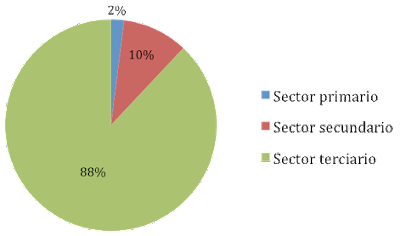
\includegraphics[width=0.5\textwidth]{sectoresEconomicosCanarias.png}
    \caption{Distribución de la masa de trabajadores entre los diferentes sectoress laborales en Canarias en el año 2020. \href{https://www3.gobiernodecanarias.org/medusa/ecoblog/jmhergare/2020/04/14/sociales-los-sectores-economicos/}{Origen de los datos}}
    \label{fig:mapaCompleto}
\end{figure}

Y en el siguiente diagrama, se observa el aporte del turismo al PIB\footnote{\textbf{PIB}:El producto interior bruto o por sus siglas PIB, mide la producción total de bienes y servicios de un país. El PIB por lo tanto, mide el tamaño de la economía de un país, es decir, toda su riqueza económica. Cuánto mayor es el PIB de un país, mayor es su capacidad económica y por tanto, mayor es su capacidad para generar empleo e inversión.} canario.
\begin{figure}[H]
    \centering
    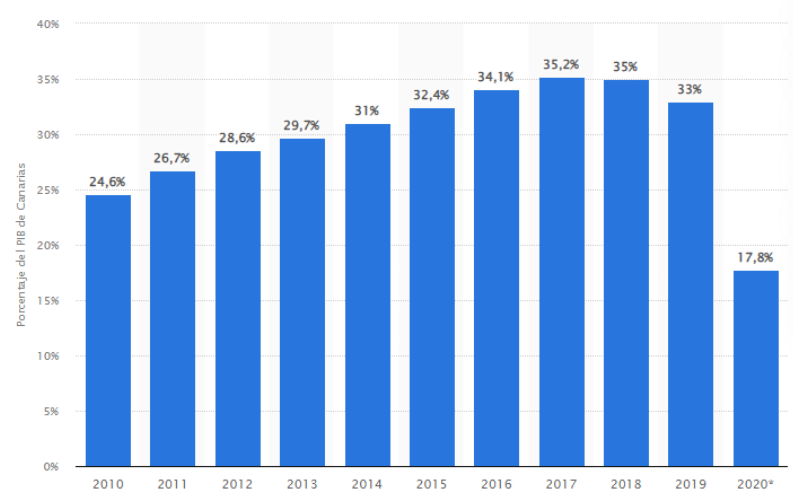
\includegraphics[width=0.5\textwidth]{pibcanarias2010-2020.PNG}
    \caption{Aporte del turismo al PIB de canarias. \href{https://es.statista.com/estadisticas/526585/aportacion-del-turismo-al-pib-de-canarias/}{Origen de los datos}}
    \label{fig:mapaCompleto}
\end{figure}

Durante los años de pandemia, ha habido un acentuado descenso en la cantidad de turistas que reciben las islas. Se estima en un 88.33\% aproximadamente entre 2019 y 2020. 


Afortunadamente, actualmente nos encontramos en un periodo de recuperación económica. 
\begin{figure}[H]
    \centering
    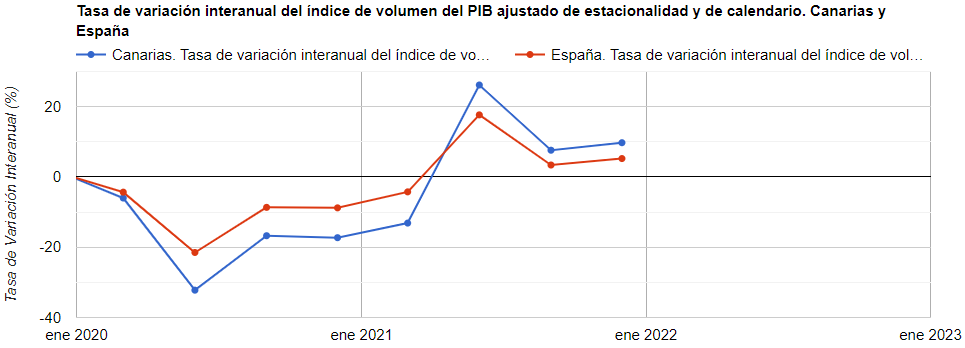
\includegraphics[width=1\textwidth]{variacionPIB2020-2022.PNG}
    \caption{Variación del PIB canario entre los años 2020 y 2022. \href{https://oic.itccanarias.org/el-pib-interanual-se-redujo-en-canarias-un-198-frente-al-87-registrado-por-el-conjunto-de-espana/}{Origen de los datos}}
    \label{fig:mapaCompleto}
\end{figure}

Este proyecto pretende dar una motivación más tanto a turistas como a residentes para visitar los diferentes puntos de la isla y así generar un mayor movimiento turístico en la zona.

%\href{http://www.gobiernodecanarias.org/istac/jaxi-istac/tabla.do?uripub=urn:uuid:ccdf465c-2230-421d-99f6-d6a1669d6032&uripx=urn:uuid:a4f8d3ed-fffc-4f58-b0bf-6ea6d2ab3d54}{info}

%\href{https://docs.google.com/spreadsheets/d/1GL6-trFgfcL-_D5phbUSWi1dCoglB_obWns4Yj6WN9Q/edit#gid=1515882426}{GoogleSheet}

\section{Justificación}

Esta aplicación puede motivar el turismo por la isla de dos maneras:\\
La primera es promocionando los sitios turísticos que se encuentran cerca del usuario, funcionando como una guía turística convencional pero con las ventajas que la plataforma móvil ofrece, como pueden ser, la disponibilidad, la actualización constante de contenido, la portabilidad etcétera.\\

La segunda es el entretenimiento que ofrece con la parte ludificada del proyecto. El mundo de los videojuegos está repleto de premios y logros que van recompensando al jugador por su curiosidad, interés y en definitiva, por seguir jugando\footnote{\href{https://www.lavanguardia.com/estilos-de-vida/20120629/54317381414/por-que-enganchan-los-videojuegos.html}{Artículo} sobre porqué las recompensas de los videojuegos nos gustan}. La aplicación presentada podría hacer que aquellos usuarios que sean coleccionistas que buscan completar todos esos premios intentasen completar el mapa de la isla, volviendo a generar movimiento por la isla.\\

Otro factor importante que puede justificar el proyecto es promover el consumo del producto de kilómetro cero\footnote{\textbf{Producto de kilómetro cero}: Los alimentos o productos de kilómetro cero son aquellos elaborados a menos de 100 km del punto de venta.} con las numerosas ventajas que ofrece este tipo de consumo.\footnote{ \href{https://grancanariamegusta.com/blog/productos-km-0-tendencia-y-concienciacion-n5}{Véase el siguiente blog del Gobierno de Gran Canaria}}. Como se comentará más adelante, sería posible incluir publicidad de establecimientos locales cercanos como pueden ser restaurantes típicos como los denominados guachinches\footnote{\textbf{Guachinche}: es un establecimiento propio de la zona norte de la isla de Tenerife, en el que se ofrece comida casera tradicional, como acompañamiento al vino de cosecha propia o de la zona a precio reducido por ser comprado directamente al productor es este.} o tiendas de artesanía típica canaria, etc. De esta forma, se favorecería un turismo orientado al consumo local, que ayudaría a las pequeñas empresas locales y al disfrute de toda la naturaleza de la isla. Gracias a tener acceso al GPS\footnote{\textbf{GPS}: Sistema de Posicionamiento Global (Global Positioning System) es un sistema que permite posicionar cualquier objeto sobre la tierra con una presición de metros o incluso de centímetros.} del dispsitivo del usuario este tipo de publicidad sería mucho más efectiva y mejor dirigida.\\

En los últimos años, este tipo de turismo parece haber aumentado en proporción al turismo más típico de "todo incluido"\footnote{\href{https://www.eldiario.es/canariasahora/turismo/canarias-no-quiere-destino-exclusivo-incluido-busca-nuevo-modelo-turistico-economia-circular_1_8164841.html}{Véase el artículo del periódico Eldiario tratando el problema del modelo de turismo de "todo incluido".}}. En los últimos años, el Gobierno de Canarias ha lanzado varias campañas para promover el cambio de modelo de turismo a uno en el que se consuman más productos locales\footnote{\href{https://rtvc.es/elaborado-en-canarias-fomenta-el-consumo-del-producto-local-en-jovenes/}{Campaña elaborado en canarias}}.

\section{Tendencia de mercado}
Como se ha comentado anteriormente, estamos actualmente, en un periodo de recuperación turística muy importante. 

\begin{figure}[H]
    \centering
    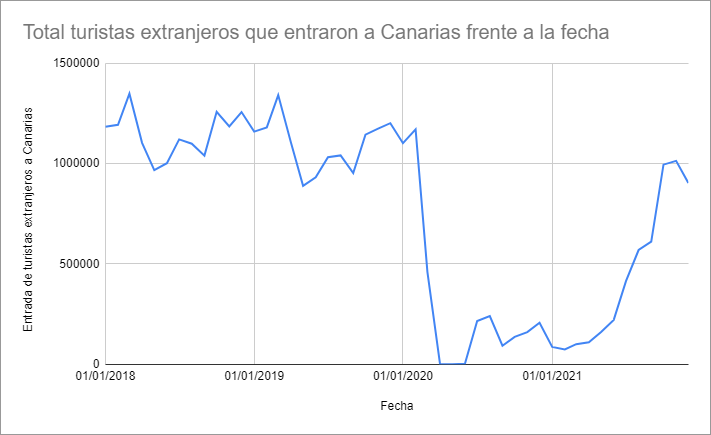
\includegraphics[width=1\textwidth]{turistas2018-2022.png}
    \caption{Gráfico que muestra la entrada de turistas extranjeros a Canarias por año. Se puede apreciar que se está comenzando a recuperar el nivel prepandémico.}
    \label{fig:mapaNoCompleto}
\end{figure}

\section{Estado actual y competencia}
Actualmente, en la Google Play Store\footnote{\textbf{Google Play Store}:  Anteriormente llamado Android Market, es una plataforma de distribución digital de aplicaciones móviles para los dispositivos con sistema operativo Android, así como una tienda en línea desarrollada y operada por Google. Esta plataforma permite a los usuarios navegar y descargar aplicaciones (desarrolladas mediante Android SDK), juegos, música, libros, revistas y películas.} podemos encontrar varias guías turísticas. 
La mayoría de estas están en formato Ebook\footnote{\textbf{Ebook}: Se trata de una versión digitalizada de un libro, algunos Ebook no tienen edición física.} lo que impide una mayor interacción por parte del usuario. Como los libros de guías turísticas tienen mayor tiempo en el mercado, éstos poseen mayor prestigio o confianza a la vista de un usuario medio. Pero, por contraparte, este tipo de guías son más difíciles de actualizar con nuevos puntos de interés.
Ya existen algunas aplicaciones que hacen de guía turística disponibles en la plataforma, pero ninguna de ellas posee ese factor de gamificación o de recompensa al usuario por visitar esos lugares, más allá del disfrute del propio lugar. A continuación, se muestra una tabla que analiza las diferencias, ventajas y desventajas de las otras guías ya disponibles en comparación con mi propuesta.

\begin{tabularx}{0.9\textwidth} { 
  | >{\centering\arraybackslash}X 
  | >{\centering\arraybackslash}X
  | >{\centering\arraybackslash}X
  | >{\centering\arraybackslash}X
  | >{\centering\arraybackslash}X | }
 \hline
 Nombre & Ventajas & Desventajas & Similitudes & Diferencias\\
 \hline\hline
 Ebooks & más experiencia y más renombre & de pago, no interactiva, sólo lectura & señala lugares de interés en la isla & no gamificado  \\
\hline
Tenerife Guia Turistica & muy buenas valoraciones en playstore, opciones para reservar en villas y hoteles, tiene navegador GPS para llegar a los lugares & no parece recordar si se ha visitado un lugar o no & señala lugares de interés en la isla & mi prototipo sólo incluirá parajes naturales o lugares públicos, no gamificado, posee opciones para visitar restaurantes \\
\hline
Mapa de tenerife offline + guia & buenas valoraciones en playstore funciona sin conexión a internet tiene descripciones de cada ubicación & no parece recordar si se ha visitado un lugar o no & señala lugares de interés en la isla & no gamificado, en la versión premium tiene sistema de navegación GPS, sistema de ubicaciones favoritas \\
\hline
Tenerife: Guía de viaje & Base de usuarios en Google Play & no parece recordar si se ha visitado un lugar o no& señala lugares de interés en la isla & no gamificado, permite planificar visitas de varios días, incluye restaurantes, hoteles y tours \\
\hline
\end{tabularx}

\section{Objetivos}
Este estudio pretende responder a las siguientes preguntas: ¿Es rentable una aplicación móvil de guía turística ludificada con estas características? ¿Ayudará realmente a incrementar el turismo por la zona?

Para responder a esas preguntas se han planteado los siguientes objetivos:

\begin{itemize}

\item Analizar las herramientas software o tecnologías disponibles para llevar a cabo el desarrollo y seleccionar la más adecuada o conveniente.

\item Identificar la competencia y establecer una serie de características con las que destacar nuestro proyecto frente a las otras soluciones disponibles.

\item Desarrollo de arquitecturas:

    \begin{itemize}
    
    \item Desarrollar un Web Scraper que capture la información de los puntos de interés.
    
    \item Implementar aplicación en android.
    
    \item Desarrollar una pagina web sencilla que permita consultar la tabla de clasificación de los usuarios.
    
        \begin{itemize}
        
        \item Se muestran los puntos de interés más cercanos a la ubicación actual del usuario.
        
        \item Se detecta cuando un usuario ha visitado un punto de interés.
        
        \item Existen opciones para permitir que el usuario decida que puntos de interés ver.
        
        \item Existen opciones para permitir al usuario elegir como se ordenan los puntos de interés; de menor distancia a mayor o de más visitados por el conjunto de usuarios a menos visitados.
        
        \end{itemize}
    
    \item Desarrollar Backend con el que conectará dicha aplicación.
    
        \begin{itemize}
            
        \item El usuario puede registrarse con email y contraseña o de forma anónima.
        
        \item La información relativa al usuario es almacenada en el servidor: qué lugares ha visitado y cuando.
        
        \item La información relativa a los puntos de interés es almacenada en el servidor: nombre, dirección, coordenadas geográficas etc.
        
        \end{itemize}
    
    \item Posible página web donde ver las puntuaciones obtenidas de los jugadores, tipo ranking.
    
    \end{itemize}
\item Realizar las pertinentes pruebas al conjunto de la aplicación.

\item Desarrollar un plan de negocio para la comercialización del producto:

    \begin{itemize}
    
    \item Crear un Diagrama de Gantt\footnote{\textbf{Diagrama de Gantt}: es una herramienta gráfica cuyo objetivo es exponer el tiempo de dedicación previsto para diferentes tareas o actividades a lo largo de un tiempo total determinado. No muestra las relaciones entre las diferentes tareas.} con las tareas a realizar, su duración, sus recursos y su costo.
    
    \item Prever la inversión inicial del proyecto.
    
    \item Diseñar modelo de comercialización del producto.
    
    \item Calcular el ROI\footnote{\textbf{ROI}: El retorno sobre la inversión (ROI, por las siglas en inglés de return on investment) es una métrica financiera que compara el beneficio o la utilidad obtenida en relación a la inversión realizada, es decir, calcula a partir de qué punto un proyecto comienza a ser rentable recuperando el dinero invertido, tanto al comienzo como durante el proceso.}.
    
    \end{itemize}
    
\end{itemize}

\chapter{Estudio Previo}
En esta sección se explicará las diferentes tecnologías o herramientas que se han barajado como opciones a la hora de desarrollar el proyecto. Además se concretará con qué tecnologías o herramientas se ha llevado a cabo finalmente el desarrollo del proyecto.
\section{Lenguaje de programación}
Hoy en día, la mayoría de aplicaciones de android se desarrollan en Kotlin\footnote{\textbf{Kotlin}: es un lenguaje de programación de tipado estático que corre sobre la máquina virtual de Java y que también puede ser compilado a código fuente de JavaScript.}, el cual ha desbancado al anterior líder del sector Java\footnote{\textbf{Java}: Es un lenguaje de programación la principal característica de Java es que es compilado a bytecode y luego, es ejecutado interpretándose en una máquina virtual, con lo cual, los programas Java sólo se compilan una vez, aun que éstos se ejecuten en diferentes sistemas.}. \textbf{[referencia a Google diciendo que preferiblemente se desarrolle en Kotlin, referencia a liderazgo de los lenguajes de programación en aplicaciones móviles]}. Los siguientes lenguajes más utilizados son JavaScript\footnote{\textbf{JavaScript}: es un lenguaje de programación interpretado. Se define como orientado a objetos, basado en prototipos, imperativo, débilmente tipado y dinámico. Se utiliza principalmente en navegadores web permitie mejoras en la interfaz de usuario y páginas web dinámicas.} y C\#\footnote{\textbf{C\#}: es un lenguaje de programación multiparadigma desarrollado y estandarizado por la empresa Microsoft como parte de su plataforma .NET}. A continuación se compararán los beneficios y defectos de cada uno de los lenguajes.
\begin{itemize}
\item \textbf{Kotlin}: De sintáxis sencilla y moderna, se ejecuta en una máquina virtual de Java\footnote{\textbf{Máquina virtual de Java}: Es una máquina virtual ejecutable en una plataforma específica, capaz de interpretar y ejecutar instrucciones expresadas en el bytecode Java, el cual es generado por el compilador del lenguaje Java.}, con lo que permite que los programas se ejecuten en cualquier plataforma que posea esta máquina virtual. \\Ventajas: Multiplataforma. \\Desventajas: Carezco de experiencia en Kotlin.
\item \textbf{Java}: Algo más complejo que Kotlin, pero al igual que kotlin, se ejecuta en una máquina virtual de Java. \\Ventajas: Multiplataforma. \\Desventajas: Carezco de experiencia en Java.
\item \textbf{JavaScript}: Potente lenguaje ampliamente utilizado en páginas web, puede usarse para crear apps en Android utilizando React Native\footnote{\textbf{React Native}: Es un proyecto de código abierto especializado en la creación de interfases de usuario. Esta plataforma permite desarrollar aplicaciones para los principales sistemas operativos, tanto móviles como de sobremesa, utilizando el entorno de desarrollo de React con las compatibilidades nativas del sistema.}. \\Ventajas: Multiplataforma, poseo experiencia en JavaScript. \\Desventajas: 
\item \textbf{C\#}: Permite crear aplicaciones multiplataforma, el mismo código se puede exportar para iOS, Android y Windows. \\Ventajas: Multiplataforma, poseo experiencia en C\#. \\Desventajas: 
\end{itemize}

\section{Entorno de desarrollo}
\begin{itemize}
\item \textbf{Unity}: pese a ser un motor de desarrollo de videojuegos, presenta utilidades y herramientas que facilitan el desarrollo de una app de estas características.
\item \textbf{Android Studio}: es el entorno de desarrollo integrado oficial para la plataforma Android. Fue creado específicamente para crear aplicaciones en Android.
\item \textbf{Microsoft Visual Studio}: es compatible con múltiples lenguajes de programación, permite a los desarrolladores crear sitios y aplicaciones web, así como servicios web en cualquier entorno compatible con la plataforma .NET.
\item \textbf{Visual Studio Code}: es un editor de código fuente desarrollado por Microsoft. Incluye soporte para la depuración, control integrado de Git, resaltado de sintaxis, finalización inteligente de código, fragmentos y refactorización de código.
\end{itemize}

\section{Plataforma para el backend}
\begin{itemize}
\item \textbf{Firebase}: es una plataforma para el desarrollo de aplicaciones web y aplicaciones móviles, está alojada en la nube y permite a los desarrolladores: sincronizar fácilmente datos de usuarios, usar herramientas multiplataforma, usar la infraestructura de Google, la cual, escala automáticamente, autentificación de usuarios, almacenamiento en la nube, etc. Todas estas ventajas abstraen al desarrollador de la parte compleja del desarrollo de un servidor. Es gratuito hasta cierto límite de usuarios.
\item \textbf{Heroku}: es una plataforma de computación en la nube que soporta distintos lenguajes de programación. Para usarlo, habría que elegir JavaScript como lenguaje de programación porque no es compatible con C\#. 
\end{itemize}

\section{Elección final del entorno de desarrollo}
Finalmente, para el desarrollo del grueso del proyecto, se ha decidido utilizar las siguientes herramientas:
\begin{itemize}
\item \textbf{Lenguaje de programación}: C\#.
\item \textbf{Entorno de desarrollo}: Unity y Visual Studio Code.
\item \textbf{Backend}: Firebase.
\item \textbf{Control de versiones}: Git\footnote{\textbf{Git}: es un software de control de versiones pensando en la eficiencia, la confiabilidad y compatibilidad del mantenimiento de versiones de aplicaciones. Su propósito es llevar registro de los cambios en archivos incluyendo coordinar el trabajo que varias personas realizan sobre archivos compartidos en un repositorio de código.} y Github\footnote{\textbf{GitHub}: es una plataforma de desarrollo colaborativo para alojar proyectos utilizando el sistema de control de versiones Git. Se utiliza principalmente para la creación de código fuente de programas de ordenador.}.
\end{itemize}
Principalmente se han elegido esas herramientas porque resultan adecuadas para el desarrollo del proyecto y además he trabajado previamente en ellas. \\
Cabe destacar que para la creación del webscraper se ha utilizado Python\footnote{\textbf{Python}: es un lenguaje de programación interpretado cuya filosofía hace hincapié en la legibilidad de su código. Es un lenguaje interpretado, dinámico, orientado a objetos y multiplataforma.} y la librería Selenium\footnote{\textbf{Selenium}: es un entorno de pruebas de software para aplicaciones basadas en la web. Permite automatizar pruebas para comprobar la interfaz de usuario de una página web.}. También se ha utilizado Python para generar un script que señala los lugares de interés repetidos para su posterior tratamiento manual y JavaScript para añadir a los puntos de interés qué zona de la isla pertenecen, ya que esto se hizo a posterior de tener la información de todos los puntos de interés.

\section{Elección de herramientas para generar la documentación}
La memoria del proyecto ha sido generada con \LaTeX{} utilizando la herramienta online \href{http://www.overleaf.com}{Overleaf}
La documentación del código fuente ha sido generada con \href{https://www.doxygen.nl/index.html}{Doxygen}.

\chapter{Desarrollo de arquitecturas}
\section{Código fuente del web scrapper}
El web scrapper que ha rastreado internet para extraer la información de los lugares de interés ha sido programado en Python utilizando la librería selenium.\\
Su código fuente es un script sencillo con el que se simula que un usuario está navegando por internet con el navegador de Google Chrome. Pero, básicamente, éste ha buscado en Google Maps y ha recolectado la siguiente información de cada lugar:
\begin{itemize}
    \item Nombre.
    \item URL de la foto.
    \item Dirección.
    \item Coordenadas geográficas.
\end{itemize}
Toda la información recolectada la ha almacenado en un fichero de texto en formato JSON.

Además he programado otro script, en JavaScript para ser ejecutado con nodeJS, que primero descartaba los sitios que tengan el mismo nombre, ya que presumiblemente serán el mismo lugar. Luego, con los que no haya descartado, les asigna a cada uno la zona a la que pertenezca mirando sus coordenadas geográficas.\\
Las divisiones en zonas de la isla será definidas en su propia sección dentro del quinto capítulo. 
\section{Estructura código fuente de la aplicación}
Para el desarrollo del código fuente de la aplicación se ha seguido el paradigma de programación orientado a objetos y eventos, ya que este es el modelo con el que trabaja Unity. Además, para cada pantalla se han utilizado diferentes escenas, las cuales serán explicadas a continuación.\\
\subsection{Escenas}
\textbf{Añadir capturas de pantalla de cada una!}
\begin{itemize}
\item \textbf{Login}: Pantalla sencilla con 4 botones que dirigen a los diferentes métodos de inicio de sesión o de registro.
\item \textbf{Inicio de sesión anónimo}: Pantalla con 2 botones y un texto explicativo de los inconvenientes de utilizar este método de inicio de sesión. Un botón permite iniciar sesión y el otro regresar a la pantalla anterior.
\item \textbf{Inicio de con Email}: Pantalla con 2 botones y 2 cuadros donde insertar texto. En el primer cuadro se espera que se introduzca un correo electrónico que tenga un formato válido para la siguiente expresión regular: cualquier caracter que no sea @ o espacio seguido de un @ seguido de cualquier caracter que no sea @ o espacio seguido de un punto y que termine con cualquier cosa que no sea @ o espacio. En el otro cuadro se debe escribir la contraseña asociada con dicho correo electrónico. Los botones, al igual que en la pantalla anteriormente descrita, permiten iniciar sesión o regresar a la pantalla anterior.
\item \textbf{Registro}: Pantalla con 2 botones y 3 cuadros donde insertar texto. Al igual que en la pantalla anteriormente descrita, en el primer cuadro se espera que se escriba un correo electrónico válido, en el segundo una contraseña para asociar con ese correo electrónico y en el tercero debe escribirse lo mismo que en el segundo cuadro. Los botones, al igual que en la pantalla anteriormente descrita, permiten iniciar sesión, esta vez creando una cuenta nueva, o regresar a la pantalla anterior.
\item \textbf{Principal}: En esta pantalla encontramos diferentes elementos. Un botón que nos llevará a la sección de ajustes, un texto que nos indica en qué zona de la isla estamos y dos barras de experiencia, una indica el porcentaje de lugares visitados dentro de la zona actual y el otro indica el porcentaje de lugares visitados de toda la isla.
\item \textbf{Lugar}:
\item \textbf{Opciones}:
\item \textbf{Estadísticas}:
\end{itemize}

\subsection{Clases Principales}
\begin{itemize}
\item \textbf{firebaseHandler}: Se encargada de manejar todos los eventos o funciones relacionadas con la base de datos Firebase, el backend de la aplicación. Es decir, contiene métodos para crear nuevos usuarios o para iniciar sesión con cada uno de los métodos permitidos. Además, almacena la información del usuario cuando éste inicia sesión, la información relativa al usuario es almacenada con un objeto de la clase \textbf{UserData}. La instancia de esta clase es única por cada ejecución y permanece entre escenas.
\item \textbf{UserData}: Es la encargada de almacenar toda la información relativa al usuario una vez ha iniciado sesión. Se almacena el identificador de usuario, los sitios que ha visitado y el nombre que posee.
\item \textbf{Place}: Se encarga de almacenar la información relativa a un punto de interés, por lo tanto en tiempo de ejecución existirán varias intancias de esta clase. Posee un método para realizar la descarga de la imagen a través de internet.
\item \textbf{gpsController}: Se encarga de gestionar el acceso al sistema GPS del dispositivo. Además, tiene métodos para verificar que los permisos de acceso al sistema GPS han sido concedidos. La instancia de esta clase permanecerá entre la pantalla principal y la pantalla de un lugar concreto.
\item \textbf{optionsController}: Se encarga de almacenar la configuración actual que el usuario ha escogido, también refleja esos cambios en la pantalla de opciones. La instancia de esta clase permanecerá entre la pantalla principal, la pantalla de un lugar concreto, la pantalla de opciones y la pantalla de estadísticas del usuario.
\item \textbf{MapRulesHandler}: Esta clase contiene atributos y métodos únicamente estáticos. No está pensada para ser instanciada, se comporta como un almacén para la información que sólo variará si se cambia la zona del planeta en la que trabaja la aplicación.
\end{itemize}

Recordar que la documentación del código fuente se encuentra en el siguiente \textbf{enlace a doc de doxygen}, allí se explica más detalladamente de qué funciones se encarga cada clase.


\section{Estructuración de la base de datos}
La estructura de la base de datos es la siguiente:
\begin{itemize}
\item \textbf{Lugares}: Tiene una entrada por cada tipo de punto de interés.
\begin{itemize}
\item  \textbf{Playas}, \textbf{miradores}, \textbf{rutas de senderismo}, \textbf{parques naturales} y \textbf{piscinas naturales}.\\ A su vez, cada una de estas categorías almacena, utilizando un identificador numérico, la información de cada punto de interés. Por lo tanto, la clave de cada punto de interés sería la tupla: tipo de sitio de interés e identificador numérico.\\
La información almacenada de cada punto de interés es:
\begin{itemize}
\item La \textbf{dirección}, si el sitio no posee dirección se rellena el campo con las coordenadas geográficas.
\item \textbf{Link a la imagen} del lugar, para la futura descarga de la imagen.
\item \textbf{Latitud} del punto geográfico donde se encuentre el punto de interés.
\item \textbf{Longitud} del punto geográfico donde se encuentre el punto de interés.
\item \textbf{Nombre} del lugar.
\item \textbf{Número de veces} que ha sido visitado.
\item \textbf{Zona} en la que se encuentra.
\end{itemize}
\end{itemize}
\item \textbf{Usuarios}: Almacena una entrada por cada usuario. Donde la clave es el UID\footnote{\textbf{UID}: Siglas de User ID, ID es la breviación de la palabra Identification. Traducido al español significa: Identificador de Usuario} del usuario
\begin{itemize}
\item \textbf{Display name}: nombre del usuario.
\item \textbf{Places Visited}: Lista ordenada cronológicamente por la \textbf{primera} visita que ha realizado dicho usuario a ese lugar. La clave es un identificador númerico que indica el orden cronológico de la primera visita. Se almacenan los siguientes valores:
\begin{itemize}
\item Identificador numérico del lugar.
\item El tipo del lugar.
\item Última vez que ese usuario ha visitado ese lugar.
\item Cuántas veces ha visitado ese usuario ese punto.
\end{itemize}
\end{itemize}
\end{itemize}

\subsection{Reglas de seguridad de la base de datos}
Una vez establecida la estructura de la base de datos, el siguiente paso ha sido establecer unas reglas de seguridad apropiadas. Las reglas que se han establecido son:
\begin{itemize}
\item Cualquier petición de un usuario no identificado se rechaza.
\item Todos los usuarios autentificados pueden leer la información de los sitios de interés.
\item Todos los usuarios autentificados pueden sobreescribir el valor de la propiedad "número de veces visitado" de todos los sitios de interés.
\item En la parte de usuarios, los usuarios sólo pueden leer y escribir la información de su propia entrada, excepto las listas de acceptedFriends, deletedFriends y challenges, las cuales pueden modificar tanto las suyas como las de otros usuarios. Esto es así para permitir establecer relaciones de amistad, eliminar relaciones de amistad o retar a otros jugadores.
\end{itemize}
Con estas reglas, se les permite a los usuarios autentificados leer toda la información de los sitios de interés pero sólo escribir el único campo que depende de ellos, el número de veces visitado. Y se impide que los usuarios puedan escribir en los campos de otros usuarios excepto los que son necesarios\\
También es importante destacar que existe unas listas; usersThatAllowFriendshipsInvitations, usersThatAllowBeChallenged, usersThatAllowAppearedOnRanking, en las cuales están apuntados los id de usuario de cada usuario que permite; recibir invitaciones de amistad, ser retado por sus amigos o aparecer en el ranking. Cada usuario puede elegir si estar o no en cada una de esas listas en el menú de opciones.
\subsection{Métodos de autenticación}
La gestión de usuarios es otra herramienta que ofrece Firebase, para este proyecto se ha decicido utilizar los siguientes métodos de autentificación:
\begin{itemize}
\item \textbf{Correo electrónico y contraseña}: Introduciendo un correo electrónico y una contraseña de, al menos, seis dígitos de longitud un usuario puede registrarse e iniciar sesión.
\item \textbf{Inicio de sesión con Google}: Utiliza una sesión iniciada previamente de una cuenta Google del dispositivo, es la opción más segura y recomendada.
\item \textbf{Inicio de sesión anónimo}: Este método que incluye firebase consiste en generar un User ID para esa instancia de ese dispositivo, es decir, si se borra los datos de la aplicación, se desinstala la aplicación y luego se instala de nuevo o si se cambia de terminal movil, se perderá la información del usuario. Este método sólo está recomendado para un primer contacto con la app, puesto que fácilmente se puede perder el progreso conseguido.
\end{itemize}
\chapter{Concepto de ludificación}

En este capítulo definiremos qué es la ludificación, también conocida como "gamificación" por su anglicismo \textit{gamification}, sus aspectos más importantes y porqué resulta una herramienta útil para incrementar la participación de los usuarios.\\

La ludificación es el uso de técnicas y elementos propios de los juegos o de los videojuegos en otro tipo de actividades para potenciar la participación y motivación de quienes realizan dichas actividades. Ejemplo de elementos de ludificación serían, puntuaciones, rangos diferenciados de nivel de progreso, tablas de clasifiación o división de las actividades en retos que van otorgando recompensas o reconocimientos al trabajo de los participantes, etcétera. Es importante, para que la ludificación tenga éxito, que los usuarios sean conscientes de su progreso. Por ello se han implementado algunas recompensas que otorgan al usuario una retroalimentación\footnote{\textbf{retroalimentación}: feedback en inglés, hace referencia a dar información sobre el resultado de una acción, en este caso concreto, para que el usuario sea consciente de que ha obrado bien y ha progresado dentro de la aplicación.} positiva.\\

El factor competitivo resulta de suma importancia a la hora de incentivar la participación y motivación de los usuarios. El hecho de estar en un entorno competitivo hace que las personas se esfuercen por destacar y por mejorar. Este fenómeno está relacionado con una necesidad que tiene el ser humano de pertenecer a un grupo ganador o sentir que su esfuerzo tiene valor.
\href{https://www.areahumana.es/personalidad-competitiva/}. Aun que, por otra parte, si el individuo no percibe progreso a pesar de su esfuerzo puede generar sentimientos de frustración. Por lo tanto, es importante que en todo momento el usuario sea consciente de que está progresando y superando a otros dentro del sistema de juego establecido.\\
Por ello, se han creado rangos de poder, tablas clasificatorias y formas de retar a otros usuarios dentro de la aplicación. Estos aspectos se explicarán en el siguiente apartado.\\

\chapter{Ludificación del proyecto}
En este capítulo es explicará la parte ludificada de la aplicación, es decir, los factores gamificados, las reglas y las recompensas.
\section{Reglas para conseguir puntuación}
Las reglas para conseguir puntuación son las siguientes:
\begin{itemize}
\item \textbf{Considerar un punto de interés como visitado}: Para que un usuario pueda registrar un punto de interés como visitado, debe estar físicamente a menos de \textbf{50 metros} de ese punto de interés, además, el usuario debe entrar en la aplicación, seleccionar ese punto de interés y tratar de registrar su visita haciendo click en el botón habilitado para ello. Para calcular la distancia a dicho punto de interés, el usuario debe tener activada la ubicación mediante servicio GPS de su dispositivo móvil y conceder los consecuentes permisos a la aplicación. Conexión a internet no es necesario porque se ha habilitado una opción de visita offline.
\item \textbf{Tiempo de espera para volver a visitar un punto de interés}: Se ha establecido que para volver a registrar un punto de interés como visitado se debe esperar al menos \textbf{una hora de tiempo real}. 
\end{itemize}

La puntuación asociada a cada acción son las siguientes:\\
\begin{itemize}
\item 10 puntos por visitar un sitio ya visitado
\item 15 puntos por visitar un sitio no visitado
\item Siempre que se visite un sitio se obtendrá una puntuación extra que será mayor cuanto menos visitado esté ese lugar. Esa puntuación extra se consigue a través de un factor multiplicativo que cumple con la siguiente fórmula:\\
\[2 - (nvl+1)/(nvm + 1)\]\\donde:\\
\textbf{nvl}: es Número de Visitas de ese Lugar que se está visitando.\\ 
\textbf{nvm}: es Número de Visitas Máximo, es decir el número de visitas que tiene el lugar más visitado de todos.\\
\\
Nótese que como máximo el factor multiplicativo será 2 y como mínimo será 1. Por lo tanto, si visitamos un lugar sin visitas y es la primera vez que lo visitamos, obtentremos 15 * 2, es decir 30 puntos.
\item Cumplir un reto. Al cumplir un reto, el usuario obtendrá la puntuación descrita en el apartado anterior y además, se le sumará el resultado de la siguiente fórmula:\\
\[(2 - (ct-st)/(mt-st))*dub\]
Donde:\\
\begin{itemize}
    \item \textbf{ct}: Completation Timestamp, es decir, el momento exacto en el que se está cumpliendo el reto.\\
    \item \textbf{st}: Start Timestamp, es decir, el momento exacto en el que el reto fue enviado.\\
    \item \textbf{mt}: Maximum Time, es decir, el plazo máximo que tienen los usuarios para completar un reto.\\
    \item \textbf{dub}: Distance to User Base, es decir, la distancia en kilómetros que separan la base del usuario del punto que está visitando.\\

\end{itemize}
\\
Como se puede observar, el resultado será, como máximo el doble de la distancia en kilómetros a la base del usuario y como mínimo esa distancia exactamente. La fórmula está construida de tal manera que el usuario obtendrá mayor puntuación cuanto más rápido complete el reto y cuanto más lejos de su base se encuentre el punto de interés que está visitando.\\

\item Cuando un usuario completa un reto, el amigo que le envió ese reto también recibe un pequeño porcentaje del total de la puntuación recibida. Ese porcentaje se ha establecido en un 10\%. 
\end{itemize}
\\
\\
Todos los parámetros y fórmulas referentes a la obtención de puntuación, para facilitar su modificación, están definidos dentro de la clase gameRules.

\section{División de la isla por zonas dentro de la aplicación}
Hemos decidido dividir la isla en  \textbf{cinco zonas} o sectores, los cuales, cuatro de ellos coinciden con los puntos cardinales, Norte, Sur, Este y Oeste. Pero además, se ha añadido un sector central.\\
Cada zona se ha determinado por las coordenadas geográficas de dicho rectángulo. A continuación, se mostrarán las coordenadas de cada zona:\\\\
\begin{tabularx}{0.9\textwidth} { 
  | >{\raggedright\arraybackslash}X
  | >{\raggedright\arraybackslash}X
  | >{\raggedright\arraybackslash}X
  | >{\raggedright\arraybackslash}X
  | >{\raggedleft\arraybackslash}X | }
    \hline
    Nombre Zona & \multicolumn{2}{|c|}{Esquina inferior izquierda} & \multicolumn{2}{|c|}{Esquina superior derecha}\\
    \hline
    \hline & latitud & longitud & latitud & longitud\\
    \hline Norte  & 28.40631 & -16.93788 & 28.60634 & -16.11673\\
    \hline Oeste  & 28.14750 & -16.93788 & 28.40631 & -16.67719\\
    \hline Centro & 28.14750 & -16.67719 & 28.40631 & -16.53193\\
    \hline Este   & 28.14750 & -16.53193 & 28.40631 & -16.11673\\
    \hline Sur    & 27.99321 & -16.93788 & 28.14750 & -16.11673\\
    \hline 
\end{tabularx}
\\
Nótese que al tratarse de divisiones rectangulares, sólo con saber las coordenadas de dos esquinas opuestas diagonalmente podemos determinar si un punto está dentro de una zona o no. Para determinar en qué zona de la isla está cada punto de interés se han utilizado las coordenadas geográficas de dicho punto.\\

Para facilitar que el usuario sea consciente del progreso que ha llevado en la aplicación, dentro de la ventana de ajustes, existe la opción de acceder a la pantalla de puntuaciones. En esta pantalla, el usuario verá una imagen de la isla con fondo blanco y con las zonas, previamente explicadas, señaladas y enmarcadas dentro de rectángulos rojos.\\

\begin{figure}[H]
    \centering
    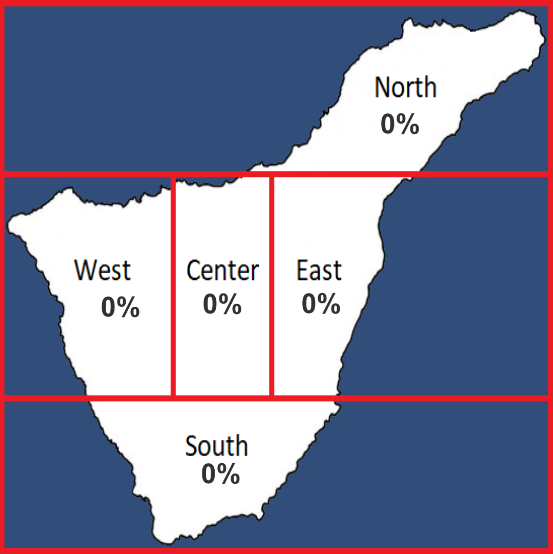
\includegraphics[width=0.25\textwidth]{mapaNoCompleto}
    \caption{Demostración de cómo se verá el mapa cuando no se haya realizado ninguna visita.}
    \label{fig:mapaNoCompleto}
\end{figure}

Además las zonas se irán rellendando, proporcionalmente a la cantidad de puntos de interés visitados dentro de esa zona, de un color azul.\\
\begin{figure}[H]
    \centering
    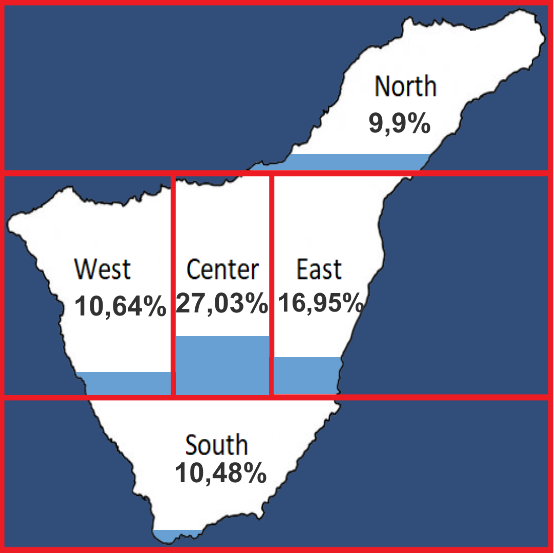
\includegraphics[width=0.25\textwidth]{mapaParcial}
    \caption{Demostración de cómo se verá el mapa cuando se haya visitado cierta cantidad de puntos de cada zona.}
    \label{fig:mapaParcial}
\end{figure}

\begin{figure}[H]
    \centering
    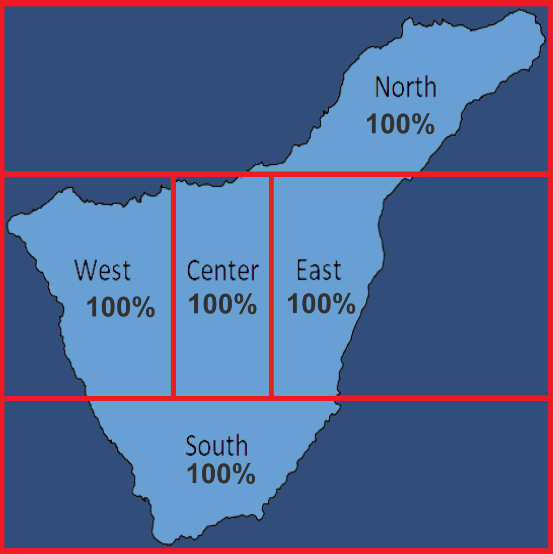
\includegraphics[width=0.25\textwidth]{mapaCompleto}
    \caption{Demostración de cómo se verá el mapa una vez se hayan visitado todos los puntos de interés de la isla al menos una vez}
    \label{fig:mapaCompleto}
\end{figure}

En la misma pantalla es posible observar diferentes estadísticas del usuario, como son:
\begin{itemize}
\item Número \textbf{total} de visitas realizadas, contabilizando varias visitas a un mismo punto.
\item Número de puntos de interés \textbf{diferentes} visitados.
\item La \textbf{zona} de la isla más visitada.
\item El \textbf{tipo} de sitio de interés más visitado
\item El \textbf{sitio} de interés más visitado de todos.
\end{itemize}

\begin{figure}[H]
    \centering
    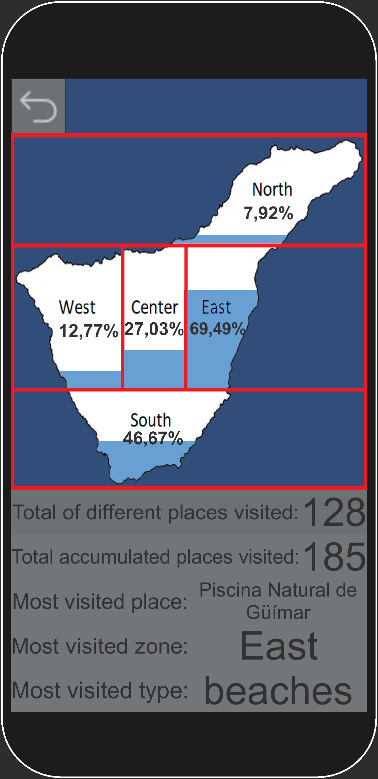
\includegraphics[width=0.25\textwidth]{pantallaEstadisticas}
    \caption{Pantalla de las estadísticas ejecutándose en un emulador}
    \label{fig:pantallaEstadísticas}
\end{figure}
\textbf{Esta captura de pantalla habría que hacerla de nuevo pero que muestre datos reales en plan has visitado 15 sitios diferentes etc.}

\newpage
\section{Recompensas}
\subsection{Rangos por nivel}
Los rangos de nivel dentro de la aplicación también presentan una forma de recompensar al usuario, haciéndole conocedor de su progreso gracias a la distinción de otros usuarios con menor rango.\\
Para establecer los rangos de nivel dentro de la aplicación se han utilizado los nombres de los diferentes niveles sociales que tenían los guanches\footnote{\textbf{Guanches}: Guanche es el nombre que se aplica a los antiguos aborígenes de la isla de Tenerife, Canarias, España, quienes la habitaban antes de la conquista castellana en 1496. Se trata de uno de los pueblos aborígenes de Canarias entroncados genética y culturalmente con los bereberes del norte de África.}.\\

La sociedad guanche era patriarcal\footnote{Información relativa a la estructura social de los guaches ha sido extraída del siguiente \href{http://www.tenerife-guanches.com/sp/sociedad.aspx}{enlace}.}, dividida en grupos sociales definidos por la riqueza, fundamentalmente la tierra y el ganado, en Tenerife existía una nobleza aborigen que esta compuesta por:
\begin{itemize}
\item \textbf{Mencey} rey o monarca de cada territorio de la isla o de la isla entera
\item \textbf{Achimencey} o gobernador, noble conformado en castas privilegiadas tanto en el ámbito político como religioso, participa en la toma de decisiones del gobierno
\item \textbf{Guañameñes} o Guadameñas , sumos sacerdotes de los Menceyatos
\item \textbf{Tagoreros} o Chaureros, corregidores y administradores de los diferentes Auchones
\item \textbf{Sigoñes} o capitanes
\item \textbf{Cichiciquitzos} o los guerreros, destinados al manejo de las armas
\item \textbf{Achicaxna} o personal dedicado a la ganadería y la agricultura
\item \textbf{Achicaxnais} dedicados a las tareas domésticas (Molineros, pescadores, alfareros, etc). 
\item Embalsamadores eran las clases más bajas.
\end{itemize}

\begin{tabularx}{0.9\textwidth} { 
  | >{\raggedright\arraybackslash}X
  | >{\raggedright\arraybackslash}X
  | >{\raggedright\arraybackslash}X
  | >{\raggedleft\arraybackslash}X | }
    \hline Nombre Rango & Puntuación mínima\\
    \hline \textbf{Mencey}         &  50.000\\
    \hline \textbf{Achimencey}     &  10.000\\
    \hline \textbf{Guañameñe}      &   3.000\\
    \hline \textbf{Tagorero}       &   1.500\\
    \hline \textbf{Sigoñes}        &     750\\
    \hline \textbf{Cichiciquitzos} &     300\\
    \hline \textbf{Achicaxna}      &     100\\
    \hline \textbf{Achicaxnais}    &       0\\
    \hline 
\end{tabularx}
\\
\\
\begin{figure}[H]
    \centering
    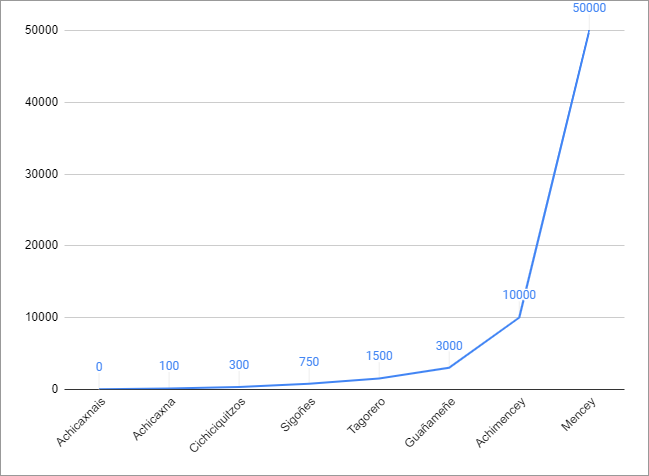
\includegraphics[width=1\textwidth]{rangosGrafico.png}
    \caption{Diagrama que muestra el incremento de la puntuación requerida para pertenecer a un rango}
    \label{fig:puntosPorRango}
\end{figure}
Hay que destacar que, en el diseño de rangos, se ha buscado hacer que los rangos más bajos estén menos distanciados en cuanto a puntuación. Esto es así para hacer que los usuarios nuevos sientan que están progresando rápidamente cuando lleva poco tiempo usando la aplicación, de esta manera se consigue que los usuarios se familiarizen rápidamente con el sistema de rangos y, además, sientan cierta satisfacción por el rápido ascenso. Progresivamente, los siguientes rangos se van distanciando para hacer que, para los jugadores veteranos, siga siendo un reto moderadamente difícil e interesante subir de rango.

\chapter{Estudio de viabilidad económica}
En este capítulo se describirá el análisis económico que se ha llevado a cabo para determinar la viabilidad del desarrollo de este proyecto de manera profesional.
\section{Fuentes de ingreso}
La posibles fuentes de ingreso que se han barajado se describen en la siguiente lista:
\begin{itemize}
\item \textbf{Vender la propia app}: La solución más obvia, pero quizás no la mejor, es simplemente vender la aplicación en las tiendas digitales para móviles como Google Play Store o su equivalente en iOS, Apple Store. La barrera de tener que pagar para probar la aplicación podría reducir considerablemente el número de usuarios que participarían en la aplicación.

\item \textbf{Google ads}: Una manera de generar ingresos podría ser incluir Google Ads a la aplicación. De esta manera no perderíamos cuota de usuarios y generaríamos unos ingresos proporcionales a la cantidad de usuarios que la utilicen. Además, esta opción cuenta con otra ventaja, y es la de poder dirigir los anuncios en función de la localización del usuario. Pudiendo publicitar lugares que se encuentren físicamente cerca del usuario potenciando los efectos de esta.

\item \textbf{Publicidad de empresas locales}: Esta manera de generar ingresos consistiría en contactar con lugares de ocio de la isla, como pueden ser centros comerciales, parques de atraciones, zoológicos, etc o de gastronomía como restaurantes de comida típica canaria. Y colocarlos como punto de interés dentro del mapa de la aplicación, por lo que los usuarios verían ese punto en el catálogo de lugares y, si quisieran completar el mapa de la isla deberían, al menos, acercarce al lugar. Esto podría ser un incentivo más para que los usuarios visiten esos lugares de ocio y posiblemente generar ingresos en esos lugares o al menos, aumentar el número de personas que transitan por esa zona. Se podrían establecer contratos temporales con las marcas, y que, al finalizar el contrato ese punto de interés desapareciera del mapa del juego.

\item \textbf{Subvención del gobierno o del cabildo}: Quizás sería posible contactar con el gobierno o el cabildo de canarias para ofrecerles participar en el proyecto para fomentar el turismo en la isla. También se podría exportar fácilmente la app a otras islas o simplificarla haciendo, por ejemplo, que sea un mapa turístico detallado, de ciudades importantes como Santa Cruz de Tenerife o La Laguna, incluyendo plazas, monumentos históricos, esculturas, etc.
\end{itemize}

Cabe destacar, que se podría hacer una combinación de estas soluciones, es decir, podríamos tener la app con publicidad de Google Ads y con lugares promocionados y ofrecer a los usuarios una versión "premium" sin publicidad.

\section{Desarrollo del proyecto}

En esta sección responderemos a las preguntas: ¿Cuánto cuesta desarrollar este proyecto? ¿Cuánto tiempo tardaría en llevarse a cabo de forma profesional el proyecto? ¿Cuándo se recuperaría la inversión inicial?

Para responder estas preguntas he utilizado el software ProjectLibre\footnote{\textbf{ProjectLibre}: es un software de administración de proyectos de código abierto programado en Java.}, done he creado un proyecto, y añadiendo, los costes estimados y la duración estimada de cada tarea se ha calculado la duración estimada del proyecto, el costo estimado y el camino crítico\footnote{\textbf{Camino crítico}: es la sucesión de tareas que marcan el inicio y el fin del proyecto, por lo tanto, son las tareas que siempre que se retrasen producirán un retraso en la fecha de finalización del proyecto.} de éste\footnote{Si desea leer con mayor detenimiento la estructuración de las tareas que componen el proyecto, el archivo que las contiene está disponible en el \href{https://github.com/AaronJoseCabreraMartin/TFG-DiscoverTenerife}{GitHub del proyecto}}.

El proyecto ha sido planteado para estar dividido en cuatro etapas:
\begin{itemize}
\item \textbf{Análisis}: En esta primera etapa se llevará a cabo un estudio de mercado en el que se incluirán tareas como: desarrollo de un análisis PEST, un análisis DAFO, un estudio sobre la identificación de la competencia y un estudio de perfiles de usuarios. También se realizará un diagrama de casos de uso UML y, para finalizar esta etapa, la creación de un documento de análisis de requerimientos. Esta etapa durará un total de 45 días.

\item \textbf{Diseño}: En esta segunda etapa se realizará el diseño completo de la base de datos, la elección del hardware y software a utilizar durante el proyecto y, por último, el diseño de las reglas del juego; cuanta puntuación se obtiene por visitar un lugar, cuanta puntuación se obtiene  por completar un reto, etc. Esta etapa durará un total de 8 días.

\item \textbf{Desarrollo}: Esta segunda etapa es la más se alarga en el tiempo de todo el proyecto. En esta etapa se implementará el diseño de la base de datos realizado en el apartado anterior, se realizará todo el proceso de extracción de información de la web: creando el web scraper, realizando una limpieza de los datos obtenidos y subiendo la información correctamente estructurada a la base de datos. También se realiazará el diseño de la interfaz gráfica tanto de la página web como de la aplicación móvil. Y, la última parte, la más importante y larga en el tiempo, la creación de la página web y de la aplicación. Esta etapa dura un total de 65 días.

\item \textbf{Despliegue}: En esta última etapa se incluye la fase de pruebas intensivas a los cuatro sectores del proyecto, al servidor, a la página web, a la aplicación de android y a la aplicación de iOS. Además también se incluye la subida de la aplicación a las plataformas de descarga de aplicaciones anteriormente mencionadas, Google Play Store  y Apple Store, con el consecuente cambio a modo de producción. En este punto el proyecto comienza a generar dinero pero, también en este punto, se añaden los gastos de producción, como son el mantenimiento de Firebase y el mantenimiento de la aplicación, con actualizaciones que corrigan posibles errores etcétera.
\end{itemize}

\section{Costo y duración del proyecto}

Tras realizar los cálculos de la aproximación de la duración estimada del proyecto, he calculado que el proyecto tardaría 7 meses en terminar su etapa final de creación, el despliegue, y tendría una inversión inicial estimada de 78078.16€.

\section{Punto estimado del retorno de la inversión inicial y producción}

En esta fase del proyecto, la aplicación ya está en el mercado y se deben añadir los ingresos que se van generando y los costos de mantenimiento de esta, los cuales, no han sido contabilizados en la inversión inicial.

Para llevar a cabo esta aproximación de los ingresos generados y de los costos de mantenimiento, se ha tenido que aproximar la cantidad de usuarios activos semanales de las dos versiones de la aplicación móvil, Android e iOS, y de la página web.\\

\begin{figure}[H]
    \centering
    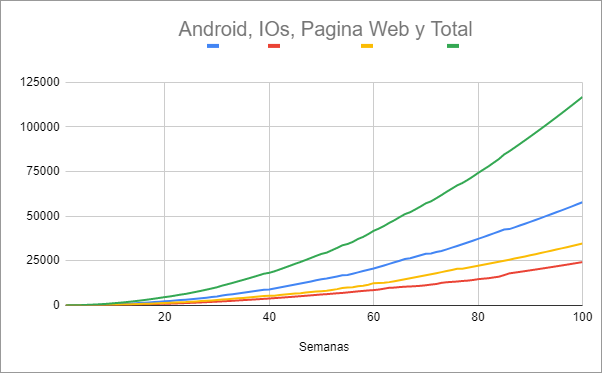
\includegraphics[width=1\textwidth]{prediccionCrecimientoUsuarios}
    \caption{Gráfico en el que se muestra la predicción del número de usuarios de cada una de las plataformas de las que consta el proyecto.}
    \label{fig:pantallaEstadísticas}
\end{figure}

Con el estudio realizado\footnote{Si desea comprobar el estudio realizado se puede comprobar en el siguiente \href{https://docs.google.com/spreadsheets/d/1Xp9dhk1jerlhGhqqkd2Uu2R6KGxOjXPJQnaUy1ktfSA/edit?usp=sharing}{enlace}.}, se ha demostrado que el proyecto alcanzaría su punto ROI\footnote{\textbf{ROI}: Retorno de Inversión, o por sus siglas en inglés Return Of Investment. Es el instante de tiempo en el cual, el dinero invertido en el proyecto se iguala con el dinero generado por el proyecto.} en la semana número 95 desde el paso a producción, es decir, se tardarían unos 23 meses en recuperar la inversión inicial. A partir de ese punto, el proyecto generaría beneficios para sus inversores. 

\begin{figure}[H]
    \centering
    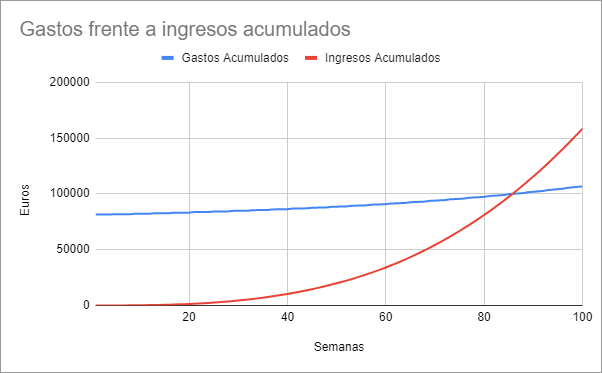
\includegraphics[width=1\textwidth]{puntoROI}
    \caption{Gráfico en el que se muestra el momento en el cual se alcanza el punto ROI}
    \label{fig:pantallaEstadísticas}
\end{figure}

Cabe señalar que no se han considerado colaboraciones con empresas locales, establecimientos de interés turístico ni subvenciones del gobierno. Estos ingresos añadidos podrían adelantar en el tiempo el punto ROI.

\chapter{Conclusiones y proyecciones futuras}
A modo de conclusión, volver a destacar la capacidad que tiene la aplicación de generar economía de kilómetro cero. Pero, no solamente haciendo publicidad de los establecimientos locales, sino que además, se podría integrar un sistema de comentarios o de valoraciones de los establecimientos publicitados, de los lugares naturales o incluso de actividades deportivas como puede ser experiencias con parapentes etc. Esto generaría una comunidad en la que los usuarios podrían compartir sus experiencias, retar a sus amigos a participar en dichas actividades o visitar esos lugares. Y, al mismo tiempo, generaría retroalimentación para las empresas.\\
\\
Gracias a la estructura del código, la aplicación podría adaptarse para funcionar con otras islas o especializarse en ciudades importantes como La Laguna o Santa Cruz de Tenerife incluyendo información sobre la historia de la ciudad, las plazas, las fuentes, etc.\\
\\
Para lograr un acabado más profesional, se debería, a la hora de registrarse con cuenta de correo electrónico y contraseña verificar el correo para evitar denegaciones de servicio. Y además, se podría añadir sistema de verificación en dos pasos y algún método de recuperación de contraseña.\\

Para añadirle mayor factor de gamificación podríamos establecer "logros" por:\\
\begin{itemize}
\item Visitar cierta cantidad de veces un mismo sitio.
\item Visitar cierta cantidad de veces todos los sitios de la zona o de la isla.
\item Acumular cierta cantidad de visitas en total de todos los sitios.
\end{itemize}

Otro posible añadido sería que los usuarios podrían tener la opción de enviar fotos y descripciones de lugares que no se encuentren dentro de la aplicación para, tras su revisión, ser añadidos al catálogo de la aplicación.\\

Como conclusión se puede extraer que durante esta memoria se ha demostrado la viabilidad económica, los múltiples beneficios y el potencial de éxito que posee este proyecto.

\chapter{Summary and conclusions}
Most of the canarian people need the comeback of the tourist situation of Canary Islands to pre-Covid levels. 
During this study we have shown how a project of a gamified touristic application could be an incentive to make people move through and discover the island. We also have shown the feasibility of make a reality this project.

We had make a marketing study and a competition study in order to increase the success probability of the project. Besides, we had created a gantt diagram that proof that the project's deployment could be completed in 7 months. We, also, had make an approximation of the quantity of user that will use both applications and the web page, and with that approximation we had calculated the profits and the costs of having the application working in production. Thanks to those calculus we had prove that the return of investment will be reached in a moderate time, 23 months.

As a conclusion, we can say that during this study we have demonstrated the viability, the benefits and the potential of this project.

\chapter{Presupuestos}

Como ya se ha indicado, el proyecto llevaría 7 meses de desarrollo. La inversión inicial ascendería a un total de 70243,4€, cabe recordar, que durante el tiempo de producción también hay gastos debido al mantenimiento del proyecto y que se tardará aproximadamente, 23 meses en recuperar la inversión inicial más el dinero invertido en el mantenimiento.

En la siguiente tabla se reflejan las horas de trabajo que supone cada tarea y el coste en €/h de cada una.\\

\begin{tabularx}{0.9\textwidth} { 
  | >{\raggedright\arraybackslash}X
  | >{\raggedright\arraybackslash}X
  | >{\raggedleft\arraybackslash}X | }
    \hline Tareas & Horas de trabajo & Costo\\
    \hline \textbf{Análisis} & 416 & 3696€\\
    \hline \textbf{Diseño} & 104 & 3535,68€\\
    \hline \textbf{Desarrollo} & 1224 & 39203,36€\\
    \hline \textbf{Despliegue} & 320 & 10324€\\
    \hline \textbf{Total} & 2064 & 65159,04€\\
    \hline 
\end{tabularx}

\end{document}
